
\documentclass{article} % For LaTeX2e
\usepackage{style,times}
\usepackage{amsmath,amsfonts,bm,amssymb}
\usepackage{algorithm}
\usepackage{algpseudocode}


%%%%% customized by shuo begin
\usepackage{amsthm,hyperref,url,dutchcal}
\usepackage{tikz,colortbl,xcolor}
\usetikzlibrary{arrows, positioning, calc, decorations.pathmorphing}
\DeclareMathOperator*{\argmax}{argmax}

\newtheorem{theorem}{Theorem}
\newtheorem{definition}{Definition}
\newtheorem{proposition}{Proposition}
\newtheorem{example}{Example}

\newcommand{\todo}[1]{\textcolor{red}{#1}}
%%%% customized by shuo end

\title{From Policy Gradient \\To Policy Proximal Policy Optimization}
\author{Shuo Liu \\
Computer Science\\
Northeastern University\\
\texttt{shuo.liu2@northeastern.edu} \\
}

\iclrfinalcopy % Uncomment for camera-ready version, but NOT for submission.
\begin{document}

\maketitle

\begin{abstract}
This article discusses PPO methods and the recent advances. 
\end{abstract}

\section{Policy Gradient (PG)}

Compared with value-based methods (Q-learning), Policy-based methods aim directly at learning the parameterized policy that can select actions without consulting a value function. PG methods seek to maximize a performance measure $J(\theta)$ with the policy's parameter $\theta$, where the updates approximate gradient ascent in $J$,\footnote{All methods following this schema are PG, whether or not they also learn an approximate value function.}
\begin{equation} \label{eq:pg}
    \theta^{(i+1)} \leftarrow \theta^{(i)} + \alpha\nabla J(\theta^{(i)}).
\end{equation}
There are 2 main advantages of PG methods,
\begin{itemize}
    \item Approximating policy can approach a deterministic policy, whereas $\epsilon$-greedy always has probability of selecting a random action;
    \item With continuous policy parameterization, the action probabilities change smoothly as a function of the learned parameter, whereas $\epsilon$-greedy may change dramatically for an arbitrarily small change in the estimated action values.
\end{itemize}

Since the major purpose of this article is to introduce PPO methods from PG, we omit some other important forms of PG here. Readers can find them in the Appendix.

\subsection{PG Theorem}

An intuitive way to calculate Equation~\ref{eq:pg} is to replace $J(\theta)$ with $V^{\pi_{\theta}} (s_0)$.\footnote{To simplify the notation, we omit $\theta$ in the subscripts, superscripts, and gradient operators, assuming $\pi$ is a function of $\theta$ and all gradients are implicit with respect to $\theta$, i.e., $V^{\pi}\equiv V^{\pi_{\theta}}$, $Q^{\pi}\equiv Q^{\pi_{\theta}}$ and $\nabla\equiv\nabla_{\theta}$.} However, the calculation is hard as it directly depends on both the action selection and indirectly the distribution of states following the target selection. PG theorem provides a nice reformulation of the derivative of the objective function to not involve the state distribution derivation.

\begin{theorem}\label{them:PG}
Taking the state-value function as the optimizing target, the objective gradient follows,
\begin{equation} \label{equ:pgthem}
    \nabla J(\theta) \propto \sum_s d^\pi(s) \sum_a Q^\pi(s,a) \nabla \pi(a|s),
\end{equation}
where $d^\pi(s)$ is the stationary distribution of the policy $\pi_{\theta}$.
\end{theorem}
To sample with expectation equals or approximates the expression Equ.~\ref{equ:pgthem},
\begin{equation} \label{equ:pgtheorem-sample}
    \begin{aligned}
        \nabla J(\theta) &\propto \sum_s d^\pi(s)\sum_a Q^\pi (s,a) \nabla\pi(a|s) \\
        &= \mathbb{E}_{d^\pi}\left[\sum_a Q^\pi (s,a) \nabla\pi(a|s) \right] \\
        &= \mathbb{E}_{d^\pi}\left[\sum_a \pi(a|s) Q^\pi (s,a) \frac{\nabla\pi(a|s)}{\pi(a|s)} \right] \\
        &= \mathbb{E}_{\pi}\left[Q^\pi (s,a) \frac{\nabla\pi(a|s)}{\pi(a|s)} \right] \\
        &= \mathbb{E}_{\pi}\left[Q^\pi (s,a) \nabla\ln\pi(a|s) \right].
    \end{aligned}
\end{equation}
The eligibility vector $\nabla\ln\pi(a|s)$ is the only place the policy parameterization appears, which can be omitted $L(\theta)=\mathbb{E}_{\pi}[Q^\pi(s,a)]$ since it will be automatically recovered when differentiating.

\subsection{PG with Baseline}

\begin{theorem} \label{them:PG-baseline}
    PG theorem can be generalized to include a comparison of the action value to an arbitrary baseline $b(s)$, as long as $b(s)$ does not depend on $a$, and this will reduce the variance while keeping it unbiased.
    \begin{equation} \label{equ:reinforce-baseline}
    \begin{aligned}
        \nabla J(\theta) &\propto \sum_s d^\pi(s)\sum_a (Q^\pi (s,a) -b(s)) \nabla\pi(a|s) \\
        &= \mathbb{E}_{\pi} \left[(Q^\pi(s,a) -b(s)) \nabla\ln\pi(a|s)\right].
    \end{aligned}
\end{equation}
\end{theorem}

According to the Theorem~\ref{them:PG-baseline}, the expected return $Q(s,a)$ in Theorem~\ref{them:PG} can be replaced by $G$ (expected return of the full or following trajectory by Monte Carlo), $A$ (advantage by Generalized Advantage Estimation or state-value prediction), and $\delta$ (TD-residual by critic prediction).


\subsection{Off-Policy PG}

Off-policy sampling reuses any past episodes, which has a higher efficiency and brings more exploration. To make PG off-policy, we adjust it with an importance weight $\frac{\pi(a|s)}{\beta(a|s)}$ to correct the mismatch between behavior and target policies. 

\begin{equation}\label{equ:pgthem-off-policy}
        \begin{aligned}  
            \nabla J(\theta) &=\nabla \left(\sum_s d^\beta(s) V^\pi(s)\right)\\
            &=\nabla\left(\sum_s d^\beta(s) \sum_a \pi(a|s) Q^\pi(s,a)\right)\\
            &=\sum_s d^\beta(s) \sum_a (\nabla \pi(a|s) Q^\pi(s,a)+\pi(a|s) \nabla Q^\pi(s,a))\\
            &\stackrel{\text{(i)}}{\approx} \sum_s d^\beta(s) \sum_a Q^\pi(s,a) \nabla \pi(a|s) \\
            &=\mathbb{E}_{d^\beta}\left[\sum_a \beta(a|s) \frac{\pi(a|s)}{\beta(a|s)}  Q^\pi(s,a) \frac{\nabla \pi(a|s)}{\pi(a|s)}\right]\\
            &=\mathbb{E}_{\beta}\left[\frac{\pi(a|s)}{\beta(a|s)}  Q^\pi(s,a) \nabla\ln \pi(a|s)\right],
        \end{aligned}
\end{equation}
where $d^\beta(s)$ is the stationary distribution of the behavior policy $\beta$, and $Q^\pi$ is the Q-function estimated regard to the target policy $\pi$. Because of hard computation in reality (i), we ignore the approximation term $\nabla Q^\pi(s,a)$. 

\newpage
\section{Proximal Policy Optimization (PPO)}

In this section, we introduce standard PPO and it variants in different domains.

\subsection{Clip-PPO}

\cite{schulman2017proximalpolicyoptimizationalgorithms} proposed the standard PPO  that uses a clipped surrogate objective to ensure the policy updates are small and controlled (proximal). Since the advantage under current policy is intangible, we can use Generalized Advantage Estimation (GAE) of the last policy to estimate $\hat{A}^{\pi_{\theta_{\text{old}}}}$ to reduce the variance of policy gradient methods and maintain low bias \cite{schulman2015gae},
\begin{equation} \label{equ:Clip-PPO}
J^{\text{CLIP}}(\theta) = \mathbb{E}_{\pi_{\theta_{\text{old}}}} \left[ \min \left( \frac{\pi_{\theta}(a|s)}{\pi_{\theta_{\text{old}}}(a|s)} \hat{A}^{\pi_{\theta_{\text{old}}}}(s, a), \text{clip}(\frac{\pi_{\theta}(a|s)}{\pi_{\theta_{\text{old}}}(a|s)}, 1 - \epsilon, 1 + \epsilon) \hat{A}^{\pi_{\theta_{\text{old}}}}(s, a) \right) \right],
\end{equation}
where $\hat{A}^\text{GAE}_t = \sum_{l=0}^{\infty} (\gamma \lambda)^l \delta_{t+l}$, $\delta$ is the TD error, and $\lambda$ is a hyperparameter controlling the trade-off between bias and variance. Note that the clipping could also occur in the value network to stabilize the training process.

The objective function can be augmented with an entropy term to encourage exploration,
\begin{equation} \label{equ:PPO}
    J^{\text{CLIP+}}(\theta) =\mathbb{E}_{\pi_{\theta_{\text{old}}}} \left[J^{\text{CLIP}}(\theta)- c\sum_{a} \pi_{\theta}(a|s) \log \pi_{\theta}(a|s))\right].
\end{equation}

\begin{algorithm}[H]
\caption{Proximal Policy Optimization (PPO)}
\begin{algorithmic}[1]
\State \textbf{Initialize}: policy parameter $\theta$ for actor network $\pi_{\theta}$, parameter $w$ for critic network $V_{w}$, replay memory $\mathcal{D}$
\For{each iteration}
    \State Generate an episode following policy $\pi_{\theta_{\text{old}}}$ and store it into $\mathcal{D}$
    \State Estimate reward-to-go $\hat{R}$ and $\hat{A}^{\pi_{\theta_{\text{old}}}}$ using GAE
        \For{each mini-batch of $N$ transitions $\{s_i, a_i, r_{i+1}, s_{i+1}\}$}
            \State Compute $J^{\text{CLIP+}}(\theta)$ for all samples according to Equ.~\ref{equ:PPO}
            \State $w \leftarrow w + \alpha_w \frac{1}{N}\sum_i\nabla_w (V_w(s_i)-\hat{R}(s_i, a_i))^2$
            \State $\theta \leftarrow \theta + \alpha_\theta \frac{1}{N}\sum_i \nabla_\theta J^{\text{CLIP+H}}(\theta)$
        \EndFor
    \State $\theta_{\text{old}} \leftarrow \theta$
\EndFor
\end{algorithmic}
\end{algorithm}

\subsection{KL-PPO}

Another formulation of PPO to improve training stability, so-called Trust Region Policy Optimization (TRPO), enforces a KL divergence constraint on the size of the policy update at each iteration \cite{schulman2017proximalpolicyoptimizationalgorithms}.
\begin{equation} \label{alg:TRPO}
\begin{gathered}
    J^{\text{KL}}(\theta) = \mathbb{E}_{\pi_{\theta_{\text{old}}}} \left[ \frac{\pi_{\theta}(a|s)}{\pi_{\theta_{\text{old}}}(a|s)} \hat{A}^{\pi_{\theta_{\text{old}}}}(s, a)-c
     \mathcal{D}_\text{KL}(\pi_{\theta_{\text{old}}} \| \pi_{\theta}) \right],
    \end{gathered}
\end{equation}
where $\mathcal{D}_\text{KL}(\pi_{\theta_{\text{old}}} \| \pi_{\theta}) = \sum_{a} \pi_{\theta_{\text{old}}}(a | s) \log \frac{\pi_{\theta_{\text{old}}}(a | s)}{\pi_{\theta}(a| s)}$.

Sometimes, the KL-penalty can be combined with policy clipping to achieve better performance in practice.

\paragraph{Adaptive-KL-PPO} \cite{schulman2017proximalpolicyoptimizationalgorithms} also mentioned Adaptive-KL-PPO, where the KL penalty coefficient is adjusted dynamically. If the policy update is too aggressive $\left( \mathcal{D}_\text{KL} \gg \mathcal{D}_\text{threshold} \right)$, $c$ is increased to penalize large updates; else if the update is too conservative $\left( \mathcal{D}_\text{KL} \ll \mathcal{D}_\text{threshold} \right)$, $c$ is decreased to allow larger updates.

\subsection{Multi-Agent PPO}

In the multi-agent setting, the PPO algorithm can be implemented independently (IPPO) or by a centralized critic (MAPPO). In IPPO, each agent has its own actor and critic and learns independently according to a joint reward \cite{ippo}. Like IPPO, MAPPO employs weight sharing between agents' critics, and the advantage in MAPPO is estimated through joint GAE \cite{mappo}.
\begin{equation} \label{equ:MAPPO}
\small
\begin{gathered}
	J^\text{IPPO}(\theta_i) = \mathbb{E}_{\pi_{\theta_{i, \text{old}}}} \left[ \min \left( \frac{\pi_{\theta_i}(a|s)}{\pi_{\theta_{i, \text{old}}}(a|s)} \hat{A}^{\pi_{\theta_{i, \text{old}}}}(s, a), \text{clip}(\frac{\pi_{\theta_i}(a|s)}{\pi_{\theta_{i, \text{old}}}(a|s)}, 1 - \epsilon, 1 + \epsilon) \hat{A}^{\pi_{\theta_{i,\text{old}}}}(s, a) \right) \right],\\
    J^\text{MAPPO}(\theta_i) = \mathbb{E}_{\pi_{\theta_{\text{old}}}} \left[ \min \left( \frac{\pi_{\theta_i}(a|s)}{\pi_{\theta_{i, \text{old}}}(a|s)} \hat{\boldsymbol{A}}^{\pi_{\theta_{\text{old}}}}(s, a), \text{clip}(\frac{\pi_{\theta_i}(a|s)}{\pi_{\theta_{i, \text{old}}}(a|s)}, 1 - \epsilon, 1 + \epsilon) \hat{\boldsymbol{A}}^{\pi_{\theta_{\text{old}}}}(s, a) \right) \right].
\end{gathered}
\end{equation}

Note that there are some other instantiations of IPPO, but not all of them are vulnerable to non-convergence issues. The one with full actor critic parameter or information sharing can be regarded as a centralized method. Besides, for cases where a general solution is still intangible even with parameter sharing (e.g. the exclusive game), heterogeneous-agent PPO allows the agents to take turns learning by using others' information, which can work well with strong assumptions.\footnote{A great example is PettingZoo's agent cycle and parallel environments.} 

\subsection{Group Relative Policy Optimization (GRPO)}

As DeepSeek has made a splash in the LLM community, the RL method GRPO involved has received a lot of attention \cite{deepseek-math}. GRPO is a variant of PPO, where the advantage is estimated using group-relative comparisons rather than GAE. This approach eliminates the critic model, which improves the training efficiency and stability. The DeepSeek framework consists of: (i) a frozen \textit{reference model}, which is a stable baseline for computing rewards; (ii) a given \textit{reward model}, responsible for evaluating generated outputs and assigning scores; (iii) a \textit{value model}, which estimates the expected return of a given state to aid in policy optimization; and (iv) a \textit{policy model}, which generates $|\mathcal{G}|$ responses and is continuously updated to improve performance based on feedback from the other components. The learning objective for GRPO is,
\begin{equation}
\small
J^\text{GRPO}(\theta) = \mathbb{E}_{\pi_{\theta_\text{old}}, i \in \mathcal{G}} \left[ \min \left( \frac{\pi_{\theta}(a_{i} | s, \vec{a}_{i})}{\pi_{\theta_\text{old}}(a_{i} | s, \vec{a}_{i})} \hat{A}^\mathcal{G}, \text{clip}(\frac{\pi_{\theta}(a_{i} | s, \vec{a}_{i})}{\pi_{\theta_\text{old}}(a_{i} | s, \vec{a}_{i})}, 1 - \epsilon, 1 + \epsilon) \hat{A}^{\mathcal{G}}\right)-c\mathcal{D}_\text{KL}(\pi_\text{ref} \| \pi_{\theta})\right],
\end{equation}
where the advantage $\hat{A}^\mathcal{G}_i=\frac{r_i-\text{mean}(r)}{\text{std}(r)}$ is estimated by grouped actions produced at the same state. $\mathcal{D}_\text{KL}(\pi_\text{ref} \| \pi_{\theta})=\frac{\pi_{\text{ref}}(a_{i} \mid s, \vec{a}_{i})}{\pi_{\theta}(a_{i} \mid s, \vec{a}_{i})} 
- \ln \frac{\pi_{\text{ref}}(a_{i} \mid s, \vec{a}_{i})}{\pi_{\theta}(a_{i} \mid s, \vec{a}_i)} - 1$ is a positive unbiased estimator, which measures the difference between the policy of trained model and reference model (like direct policy optimization).

\vspace{5mm}
\begin{figure}[h]
    \centering
    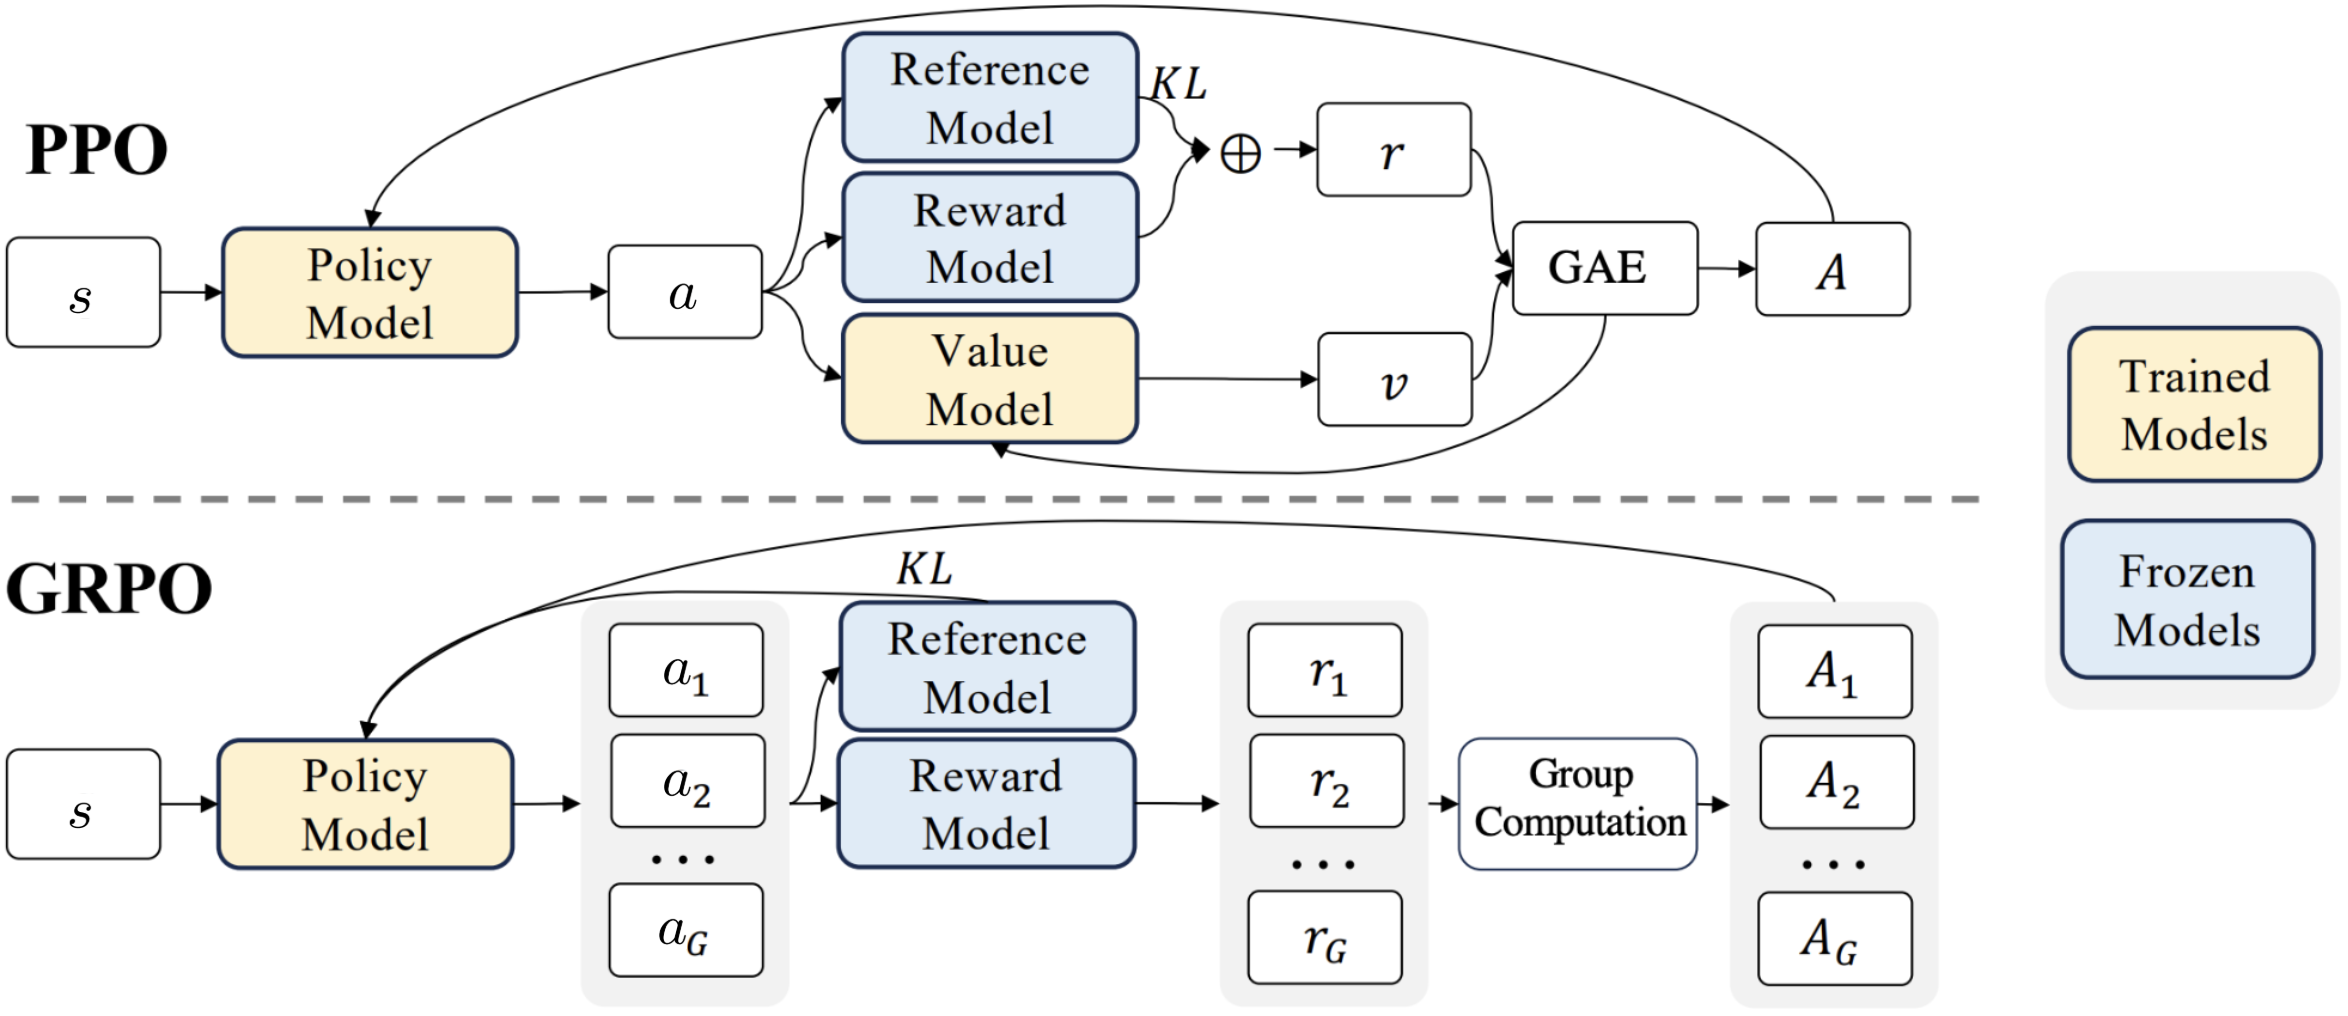
\includegraphics[width=0.8\linewidth]{grpo.png}
    \label{fig:grpo}
\end{figure}

\clearpage
\bibliography{ref}
\bibliographystyle{ref}
\newpage
\appendix
\section{Omitted Proofs}

This section shows the omitted (but non-trivial) proofs.

\subsection{Proof Theorem~\ref{them:PG}}
\begin{proof}
The gradient of $V$ function can be written in terms of $Q$ function,

{\footnotesize
    \begin{equation}
        \begin{aligned}
            \nabla V^{\pi}(s) &= \nabla\left [ \sum_a \pi(a|s) Q^\pi (s,a)\right ] \\
            &=\sum_a\left [ \nabla\pi(a|s) Q^\pi (s,a) +\pi(a|s) \nabla Q^\pi (s,a) \right] \\
            &=\sum_a\left [ \nabla\pi(a|s) Q^\pi (s,a) +\pi(a|s) \nabla \sum_{s'}P(s'|s, a)(r+V^\pi(s')) \right] \\
            &\stackrel{\text{(i)}}{=}\sum_a\left [ \nabla\pi(a|s) Q^\pi (s,a) +\pi(a|s) \sum_{s'}P(s'|s, a)\nabla V^\pi(s') \right ], \\
        \end{aligned}\nonumber
    \end{equation}
}
where we can have the derivation (i) since $r$ only depends on the environment dynamics.

Let $\phi(s) = \sum_a \nabla\pi(a|s) Q^\pi (s,a)$. We use $\rho^\pi(s\rightarrow x, k)$ to represent the probability of transitioning from state $s$ to $x$ with policy $\pi$ after $k$ steps, i.e., $\rho^\pi(s \rightarrow s', 1)=\sum_a \pi(a|s) P(s'|s, a)$. Thus, we can unroll the recursive form as below,

{\footnotesize
    \begin{equation} 
        \begin{aligned}
            \nabla V^{\pi}(s) &=\phi(s) +\sum_a \pi(a|s) \sum_{s'}P(s'|s, a)\nabla V^\pi(s') \\
            &= \phi(s) + \sum_{s'}\rho^\pi(s \rightarrow s', 1) \nabla V^\pi(s') \\
            &= \phi(s) + \sum_{s'}\rho^\pi(s \rightarrow s', 1)\left[\phi(s') + \sum_{s''}\rho^\pi(s' \rightarrow s'', 1) \nabla V^\pi(s'')\right] \\
            &= \phi(s) + \sum_{s'}\rho^\pi(s \rightarrow s', 1) \phi(s') + \sum_{s''}\rho^\pi(s \rightarrow s'', 2) \nabla V^\pi(s'')  \\
            &= \phi(s) + \sum_{s'}\rho^\pi(s \rightarrow s', 1) \phi(s') + 
             \sum_{s''}\rho^\pi(s \rightarrow s'', 2) \phi(s'') +
            \sum_{s'''}\rho^\pi(s \rightarrow s''', 3) \nabla V^\pi(s''')  \\
            & \qquad \qquad \vdots \\
            &= \sum_{k=0}^{\infty}\sum_{x}\rho^\pi(s\rightarrow x, k)\phi(x)\\
        \end{aligned}\nonumber
    \end{equation}
}

We use $\eta(s)$ to represent the expected number of visits for $s$ in a single episode (in episodic case $\sum_s \eta(s)$ is the averaged length of an episode; in continuous case $\sum_s \eta(s)=1$). By plugging it into the object function $J$,
\begin{equation}
    \begin{aligned}
        \nabla J(\theta) &= \nabla V^\pi (s_0)   \\
        &= \sum_s \left( \sum_{k=0}^\infty \rho^\pi(s_0 \rightarrow s, k) \right) \sum_a \nabla\pi(a|s) Q^\pi (s,a) & \\
        &= \sum_s \eta(s) \sum_a \nabla\pi(a|s) Q^\pi (s,a)  \\
        &\stackrel{\text{norm}}{=} \left(\sum_s \eta(s) \right) \left(\sum_s \frac{\eta(s)}{\sum_s \eta(s)} \right )\sum_a \nabla\pi(a|s) Q^\pi (s,a) \\
        &\propto \sum_s d^\pi(s)\sum_a \nabla\pi(a|s) Q^\pi (s,a)
    \end{aligned}\nonumber
\end{equation}
\end{proof}

\subsection{Proof of Theorem~\ref{them:PG-baseline}}

\begin{proof}
We first prove PG with baseline is unbiased,
    \begin{equation}
        \begin{aligned}
            &\quad\mathbb{E}_{ d^\pi}\left [\sum_a (Q^\pi(s,a) -b(s)) \nabla\ln\pi(a|s)\right]\\
            &=\mathbb{E}_{ d^\pi}\left [\sum_a Q^\pi(s,a)\nabla\ln\pi(a|s)\right] -\mathbb{E}_{ d^\pi}\left [\sum_a b(s) \nabla\ln\pi(a|s)\right]\\
            &= \mathbb{E}_{ d^\pi}\left [\sum_a Q^\pi(s,a)\nabla\ln\pi(a|s)\right] - \mathbb{E}_{ d^\pi}\left [b(s) \nabla\sum_a \ln\pi(a|s)\right]\\
            &=\mathbb{E}_{ d^\pi}\left [\sum_a Q^\pi(s,a)\nabla\ln\pi(a|s)\right] - \mathbb{E}_{ d^\pi}\left [b(s) \nabla 1\right]\\
            &=\mathbb{E}_{ d^\pi}\left [\sum_a Q^\pi(s,a)\nabla\ln\pi(a|s)\right],
        \end{aligned} \nonumber
    \end{equation}
and the variance of PG with baseline is,
    \begin{equation}
        \begin{aligned}
            &\quad \mathbb{V}_{ d^\pi}
            \left [\sum_a (Q^\pi(s,a) -b(s)) \nabla\ln\pi(a|s)\right]\\ 
            &\stackrel{\text{(i)}}{\gtrapprox} \sum_a \mathbb{E}_{ d^\pi} \left [ \left((Q^\pi(s,a) -b(s)) \nabla\ln\pi(a|s)\right)^2\right] - \left(\mathbb{E}_{ d^\pi} \left [\sum_a (Q^\pi(s,a) -b(s)) \nabla\ln\pi(a|s)\right]\right)^2 \\
             &\stackrel{\text{(ii)}}{\approx} \sum_a \mathbb{E}_{ d^\pi} \left [\left(Q^\pi(s,a) -b(s)\right)^2\right] \mathbb{E}_{ d^\pi}\left[\left(\nabla\ln\pi(a|s)\right)^2\right] - \left(\mathbb{E}_{d^\pi} \left [\sum_a Q^\pi(s,a) \nabla\ln\pi(a|s)\right]\right)^2 \\
             &< \sum_a \mathbb{E}_{ d^\pi} \left [\left(Q^\pi(s,a)\nabla\ln\pi(a|s)\right)^2\right] - \left(\mathbb{E}_{ d^\pi} \left[\sum_a Q^\pi(s,a) \nabla\ln\pi(a|s)\right]\right)^2 \\
             &\stackrel{\text{(iii)}}{\lessapprox} \mathbb{E}_{ d^\pi} \left [\left(\sum_a Q^\pi(s,a)\nabla\ln\pi(a|s)\right)^2\right] - \left(\mathbb{E}_{ d^\pi} \left[\sum_a Q^\pi(s,a) \nabla\ln\pi(a|s)\right]\right)^2 \\
             &= \mathbb{V}_{ d^\pi} \left[ \sum_a Q^\pi(s,a)\nabla \ln \pi(a|s)\right].
        \end{aligned} \nonumber
    \end{equation}
    
    In approximations (i) and (iii), we only keep the quadratic term and omit the products, but this won't affect the property of the inequality because the deduction loss caused by $\prod_a (Q^\pi(s,a) -b(s)) \nabla\ln\pi(a|s)$ is less than the increase we compensate for $\prod_a Q^\pi(s,a) \nabla\ln\pi(a|s)$. In approximation (ii), we assume independence among the values involved in the expectation for factorization. This reveals that REINFORCE has less variance when using a baseline; and when $b(s)\approx V^\pi(s)$, the variance reaches optimal.
\end{proof}

\newpage
\section{Other Forms of PG}

Since the major purpose of this article is to introduce PPO methods from PG, we omit some other important forms of PG in the main body. Here are the complements.

\subsection{Deterministic PG}

Sometimes we hope the policy function to be deterministic to reduce the gradient estimation variance and improve the exploration efficiency for continuous action space \footnote{The deterministic PG is a special case of the stochastic PG, with $\sigma=0$ in the re-parameterization $\pi_{\mu_{\theta}, \sigma}$.} (i.e., a decision $a=\mu_{\theta}(s)$). PG for a deterministic policy in continuous action space is,
\begin{equation}\label{equ:pgthem-deterministic}
        \begin{aligned}  
            \nabla_{\theta} J(\theta) &=\nabla_{\theta} \left(\int_s d^\mu(s) V^\mu(s) ds\right)\\
            &=\nabla_{\theta} \left(\int_s d^\mu(s) Q^\mu(s,a)|_{a=\mu_{\theta}(s)}ds\right)\\
            &\stackrel{\text{(i)}}{=}\int_s d^\mu(s) \nabla_{\theta} \mu_{\theta}(s) \nabla_a Q^\mu(s,a)|_{a=\mu_{\theta}(s)} ds 
            \\
            &=\mathbb{E}_{d^\mu} [ \nabla_{\theta} \mu_{\theta}(s) \nabla_a Q^\mu(s,a)|_{a=\mu_{\theta}(s)}],
        \end{aligned}
\end{equation}
The derivation (i) the state distribution is non-differentiable w.r.t. $\theta$ (i.e., derivation (i))\footnote{A small change in $\theta$ can cause a substantial change in the trajectory, and the state visitation distribution can exhibit non-smooth behavior as a function of $\theta$.}, To guarantee enough exploration of determinant PG, We can either add noise into the policy 
\begin{equation}
    \mu'(s) = \mu_{\theta}(s) + \mathcal{N},
\end{equation} 
or learn it off-policy-ly by following a different stochastic behavior $\beta(a|s)$ policy to collect samples,
\begin{equation}\label{equ:pgthem-deterministic-offpolicy}
        \begin{aligned}  
            \nabla_{\theta} J(\theta) &=\nabla_{\theta} \left(\int_s d^\beta(s) Q^\mu(s,a)|_{a=\mu_{\theta}(s)}ds\right)\\
            &=\mathbb{E}_{d^\beta} [ \nabla_{\theta} \mu_{\theta}(s) \nabla_a Q^\mu(s,a)|_{a=\mu_{\theta}(s)}],
        \end{aligned}
\end{equation}

\subsection{Distributed PG}

Due to the efficiency of the GPU-cluster in training, some workers (machines or processes) are employed in a distributed manner to generate rollouts and compute policy gradients in PG methods \cite{brenner2023ppo}. The distributed advancement can also be extended to any PG extension, like Actor-Critic (AC), PPO, and deterministic PG methods.

\paragraph{Centralized v.s. Decentralized} These workers can either share a central parameter server or update their own weights in a decentralized manner, where aggregation techniques such as AllReduce may be utilized. Rather than merely collecting rollouts and calculating the gradient according to its replay buffer, the workers can be further decentralized into \textit{agents} with their parameters, which is closely related to PG in multi-agent setting.

\paragraph{Synchronous v.s. Asynchronous} In the centralized paradigm, weight updates can be conducted synchronously, where gradients from all workers are aggregated (typically through summation or averaging) before updating the model parameters. This ensures a globally consistent update but may introduce inefficiencies due to synchronization delays. Alternatively, asynchronous updating allows each worker to update the global parameters independently, without waiting for all gradients to be collected. This method can improve computational throughput but may lead to stale gradients and slower convergence. The difference between these 2 approaches is exemplified in Advantage Actor-Critic (A2C) and Asynchronous Advantage Actor-Critic (A3C).




\end{document}
